% Please write one sentence per line! (easier for version control)
% MY IMPORTANT REMARK

\documentclass[10pt, a4paper]{article}
\usepackage{lrec2006}
\usepackage{graphicx}
\usepackage{todonotes}
\usepackage{linguex}
\usepackage{amssymb}

\title{Towards text mining in earth science:\\
extraction of quantitative variables and their relations}

\name{Author1, Author2, Author3}

\address{ Affiliation1, Affiliation2, Affiliation3 \\
               Address1, Address2, Address3 \\
               author1@xxx.yy, author2@zzz.edu, author3@hhh.com\\}


\abstract{
This paper addresses text mining in the cross-disciplinary domain of environmental science and climate science.
It is motivated by the desire for literature-based knowledge discovery from scientific publications.
The particular goal is to automatically extract relations between quantitative variables from raw text.
This results in rules of the form ``If variable X increases, than variable Y decreases''.    
As a first step in this direction, an annotion scheme is proposed to capture the events of interest -- those of change, cause, correlation and feedback -- and the entities involved in them -- quantitative variables.
Its purpose is to serve as an intermediary step in the process of rule extraction.
It is shown that the desired rules can indeed be automatically extracted from annotated text.
A number of open challenges are discussed, including automatic annotation, normalization of variables, reasoning with rules in combination with domain knowledge and the need for meta-knowledge regarding context of use.
\\ \newline 
\Keywords{Text Mining, Literature-based Knowledge Discovery, Environmental Science, Climate Science, Corpus Annotation, Relation Extraction, Event Extraction}}

\newcommand{\tag}[1]{\textsc{#1}}

% Define your own todo notes here, like 
% \newcommand{\XX}[1]{\todo[inline,author=XX,color=YY]{#1}}
\newcommand{\EM}[1]{\todo[inline,author=EM,color=yellow]{#1}}
\newcommand{\EA}[1]{\todo[inline,author=EA,color=green]{#1}}
\newcommand{\MVA}[1]{\todo[inline,author=MVA,color=blue]{#1}}
\newcommand{\PO}[1]{\todo[inline,author=PO,color=pink]{#1}}



\begin{document}

\maketitleabstract

%=============================================================================
\section{Introduction}
%=============================================================================

\todo[inline]{Argue that text mining in environmental sciences:
has not been really pursued so far;
is different from text mining in biomedicine}

\todo[inline]{Applications: search, QA, etc}.

The scientific literature is growing so rapidly that researchers have been forced to become increasingly specialized to keep up with the state-of-the-art. 
This specialization can lead to the fragmentation of science, as researchers from different (sub-)disciplines rarely have time to read each other's papers. 
\newcite{Swanson1986Undiscovered} claimed that this fragmentation of science gives rise to \emph{undiscovered public knowledge}, i.e. still unmade inferences that can be made based on publicly available knowledge. As an example, he hypothesized that fish oils can cure Raynaud's disease by combining two publicly available statements: 1) Fish oils reduce blood viscosity, 2) patients with Raynaud's disease tend to exhibit high blood viscosity \cite{Swanson1986Fishoil}. 
This method of making hypothesis inferences of the form $A \to C$ based on publicly available statements $A \to B$ and $B \to C$ has been termed \emph{Swanson linking}\footnote{In the Swanson linking paradigm, the operator $\to$ is not interpreted as a logical conditional, but rather as an abstract causal or correlative relation between the terms. The conclusion $A \to C$ is therefore not logically sound, but has nevertheless been showed to give empirically useful results.}. 

The discoveries of Swanson prompted a line of research into methods for computer support in the identification of undiscovered public knowledge, an area which has been labelled Literature-based discovery (LBD). 
Most LBD methods are based on Swanson linking, and use term co-occurrence frequencies to detect relations of the type $A \to B$. 
Terms are usually extracted as n-grams from the text \cite{Lindsay1999LBDLexicalStat} or taken from a controlled vocabulary or ontology \cite{Weeber2001ConceptsInLBD}.

Recently, co-occurrence based methods have come under critique for leading to too many spurious discoveries.
\newcite{Hristovski2008NLPinLBD} therefore advocate an approach based on Natural Language Processing (NLP), as such approaches are able to be more specific about the relation that holds between two terms. 
LBD efforts have traditionally been undertaken in the biomedical domain, and have therefore benefited from existing biomedical NLP tools such as SemRep\footnote{http://semrep.nlm.nih.gov/}.
Application of NLP-based LBD techniques to less resourced domains, such as the environmental sciences, would however require the development or adaptation of NLP tools to the new domain.

\todo[inline]{Related work (possibly in separate section or in Discussion section):
\cite{Hashimoto2012Excitatory}
\cite{Mihaila2013BioCause}
\cite{Zambach2010Lexical}
\cite{Vossen2008}}
NLP-based approaches are based on the automatic extraction of relations from text. Causal relatiosn are one of the most popular types of relations to extract. They are used not only for LBD but also for question answering. In the work by \cite{Mihaila2013}, several machine learning algorithms are applied to recognize causality triggers such as "therefore", "because", "as a result of" etc. The approach is tested on BioCause and BioDRB corpora, which consist of articles with manually annotated causal relations between named entities in the biomedical domain. Machine learning approach has also been applies by \cite{Pechsiri2010a} to extract causal relations in the agricultural domain. These relations are then used to construct explanation knowledge graphs that represent the domain knwoledge.

Causal relations is one type of relations that can be used for LBD purposes. Other, more fine-grained types of relations has been identified as well. In the work by \cite{Zambach2010Lexical}, the authors identify and analyze verbs that express regulation relations, postive and negative, between processes and substances in biomedical domain. They propose that this knowledge can be used for automatic annotation of such relations in text. A somewhat similar types of relations has been proposed by \cite{Hashimoto2012Excitatory}. They identify excitory, inhibitory and neutral relations with corresponding set of extraction templates. More templates are acquired automatically by a bootstrapiing process. Excitatory relations are then used for extraction of contradictions, causality relations and genration of causality hypothesis.

The remainder of this paper is structured as follows. 
The next Section proposes a new annotation scheme to capture the events of interest -- those of change, cause, correlation and feedback -- and the entities involved in them -- quantitative variables. 
Section~\ref{sec:extraction} shows that  rules can indeed be automatically extracted from annotated text.
Section~\ref{sec:discussion} discusses a number of open challenges are discussed, including automatic annotation, normalization of variables, reasoning with rules in combination with domain knowledge and the need for meta-knowledge regarding context of use.
The last Section closes with conclusions and future work.

%=============================================================================
\section{Annotation}
%=============================================================================

\subsection{Procedure}

The data consisted of 12 abstracts (2369 words) from recent, high-quality scientific journal publications about the relation between climate and ocean changes. 
These were selected by our domain expert (author MVA) as a reasonably representative sample of the text type in the targeted area, comprissing multi-disciplinary work in marine biology, marine science, oceanography, environmental science, climate science, biogeoscience and geophysics.
Text was automatically extracted from PDF files.
Abstracts were manually extracted, tokenized and split into sentences, also allowing for manual correction of minor PDF-to-text conversion errors.

Annotation was carried out using the Brat annotation tool \cite{stenetorp2012}.
The annotion scheme described below was developed in an iterative fashion in close colaboration with our domain expert.
It is inspired by annotation efforts in the biomedical domain such as the GENIA corpus \cite{Kim2003GENIA} and the corpora used in the BioNLP shared tasks on event extraction \cite{Kim2009Overview}.
It covers a particular type of events -- those of change, cause, correlation and feedback -- and the entities involved in them -- quantitative variables.
The primary reason of annotation is not to analyse the text according to some linguistic formalism or theory, or to follow some knowledge representation formalism or ontological theory.
Instead the purpose of the annotation is rather pragmatic: to serve as an intermediary step in the process of extracting rules about the relation between quantitative variables from raw text.      
 
The annotation scheme proposed below seems a good candidate for this purpose.
However, it remains to be seem how it holds up when applied to more text.
Inter-annotator agreement has not been measured so far.
\EM{Probably better to merge this paragraph into Discussion section} 

\subsection{Annotation scheme}

The resulting annotation scheme involves one type of entity (variable), several types of events (change, increase, decrease, cause, correlate, feedback) and some basic logic structure (and/or, negation).  


\subsubsection{Variables}

A quantitative variable is an entity that can be counted or measured.
Its value can be naturally expressed by a number such as a count, a ratio, a percentage or a scalar (quantity of units).
It can be regarded as a (potential) quantitative variable in an experiment or a model. 
Not every variable in the text is labeled as such.
To save annotation time and effort, only those variables related to a change are annotated.
The  direction of change can be positive (increasing), negative (decreasing) or unspecified (either increasing or decreasing), but there must always be a clear cue in the text that the variable is involved in some change. 
Examples of changing, increasing and decreasing variables respectively:

\ex.
  \a. significant changes in [\emph{surface ocean pH}]
  \b. rise in [\emph{atmospheric CO2 levels}]
  \c. decline in [\emph{marine primary production}]

In contract, the text spans in \Next are not annotated as variables.

\ex.
  \a. *[\emph{carbon dioxide}] and [\emph{light}] are two major prerequisites of photosynthesis
  \b. *changes in [\emph{the network of global biogeochemical cycles}] 
  \c. *The concentrations of [\emph{DFe}] and [\emph{TaLFe}] were relatively high

The text spans in \Last[a] are measurable, in principle at least, but there is no textual cue in the context indicating that they are subject to change. 
The text span in \Last[b] admittedly identifies something that is changing, but it is an abstraction -- not something that can be measured and naturally expressed through a number. 
The ones in \Last[c] express a static state rather than a dynamic event.
The reason for excluding cases like these is that they do not lead to useful rules about the relation between quantitative variables.

Variables must be indicated as precisely as possible, that is,including any relevant specifications, modifications or conditions. So instead of \Next[a], \Next[b] is prefered.

\ex.
  \a. *a difference in [\emph{carbon concentration}] between the ocean surface and the deep waters
  \b. a difference in [\emph{carbon concentration between the ocean surface and the deep waters}]

The choice is motivated by the idea that, given a syntactic parse, it is usually easier to generalize a complex argument by stripping modifiers than the other way around.  

Variables are tagged with the label \tag{Variable}. It is most likely advantaguous to distinguish different subclasses of variables. Currently we are not concerned with this. 
However, we do not exclude the possibility of a more fine-grained annotation at a later stage. 


\subsubsection{Change, Increase and Decrease}

A change is an event in which the value of a quantitative variable is changing.
The direction of change can be positive (increasing), negative (decreasing) or unspecified (either increasing or decreasing), but there must always be a clear cue in the text that the variable is involved in a change.
This is referred to as the \emph{trigger} for the event.

Examples of triggers for event types of change, increase and decrease are:

\ex.
  \a. [\emph{regional changes}] in phytoplankton
  \b. [\emph{addition of}] labile dissolved organic carbon
  \c. [\emph{to slow down}] calcification in corals

Changes must apply to a variable; hence the text span in \Next does not trigger a

\ex. *marine primary production is sensitive to climate [\emph{variability and change}]

Events of increase, decrease and undirected changes are tagged as \tag{Increase}, \tag{Decrease} and \tag{Change} respectively. 
Events are related to variables through thematic roles, which specify the different participants in the event. 
Change events must always have a \tag{Theme} role that is filled by the variable that is changing.
Typical annotation examples are therefore:\footnote{We use labeled brackets to denote enitities, events or thematic roles, depending on the context of discussion.}

\exi.
  \a. [\tag{Decrease} reduced] [\tag{Theme} calcite production]
  \b. [\tag{Change} significant changes in] [\tag{Theme} surface ocean pH]

In addition, they can optionally have an \tag{Agent} role or a \tag{Co-theme} role, which will be explained in the next Section.

Change events can also function as Cause/Correlate events, as will be described in the next Section, in which case they take an AGENT or CO-THEME role as well.


\subsubsection{Cause}

Cause events involve a pair of changes where the first change causes the second change.
Since a change event involves a changing variable, as its theme, causal events thus express a causal relation between two changing variables. 
The trigger of a cause event is annotated with a \tag{Cause} tag.
Triggers are often verbs, but can also be adjectives (\emph{stimulatory}), adverbs (\emph{therefore}) or subjunctive phrases (\emph{due to}, \emph{in response to}) and other phrasal expression (\emph{has an effect on}).  

Cause events must always have two thematic roles: an \tag{Agent} identifying the cause and a \tag{Theme} identifying the effect. 
% Notice that causal relations are directional. 
% That if, if  A causes B, then it does not follow that B causes A.
Examples of cause events are:

\exi.
  \a. [\tag{Agent} rise in atmospheric CO2 levels] [\tag{Cause} \emph{causes}] [\tag{Theme} significant changes in surface ocean pH]
  \b. [\tag{Agent} Fe(III) addition in the presence of GA (FeGA)] [\tag{Cause} \emph{gave}] [\tag{Theme} higher Fe(II) concentration]
  \c. [\tag{Agent} diminished calcification] [\tag{Cause} \emph{led to}] [\tag{Theme} a reduction in the ratio of calcite precipitation to organic matter production]
% number of examples can be reduced

In many cases, a cause event and a change event share one and the same trigger, as in the following examples:

\exi.
  \a. [\tag{Agent} changes in the magnitude of total and export production] [\tag{Change} \emph{can strongly influence}] [\tag{Theme} atmospheric CO2 levels]
  \b. [\tag{Theme} calcification and net primary production] [\tag{Increase} \emph{ are significantly increased by}] [\tag{Agent} high CO2 partial pressures]
  \c. [\tag{Agent} addition of labile dissolved organic carbon] [\tag{Decrease}  \emph{reduced}] [\tag{Theme} phytoplankton biomass]

In \Last[a], \emph{can strongly influence} serves as the cue for a change event with variable \emph{atmospheric CO2 levels} as its theme. 
At the same time, it is the trigger for a cause event with agent \emph{ changes in the magnitude of total and export production} and theme \emph{atmospheric CO2 levels}.
In principle, both events can be annotated individually.  
However, in order to avoid a needlessly complex annotation, we choose to not annotate the cause event explicitly. 
Instead \emph{changes in the magnitude of total and export production} is given the role of agent in the change event. 
Presence of an agent role suffices to infer the cause event.
Two more instances of this pattern are shown in \Last[b] and \Last[c].

\EM{Describe exceptional cases of variable with implicit change}


\subsubsection{Correlate}

Correlate events involve a pair of changes where the first change correlates with the second change. 
Since a change event involves a changing variable, as its theme, correlate events thus express a correlation between two changing variables. 
That is, if one of them changes, the other changes along. 
Correlations  have two roles, \tag{Theme} and \tag{Co-theme}, both of which should be fulfilled by a change event (i.e. \tag{Increase}, \tag{Decrease} or \tag{Change}).
% or a quantitative variable (Variable)
Examples of correlate events:

\exi.
  \a. [\tag{Theme} reduced calcite production] [\tag{Correlate} \emph{ was accompanied by}] [\tag{Co-theme} an increased proportion of malformed coccoliths]
  \b. [\tag{Theme} carbon:nutrient ratio turns out to decrease] [\tag{Correlate}  \emph{with}] [\tag{Co-theme} increasing mixed-layer depth and temperature]
  \c. Here we report [\tag{Them}e reduced calcite production] [\tag{Correlate}  \emph{at}] [\tag{Co-theme} increased CO2 concentrations]
  \d. [\tag{Correlate} \emph{When}] [Co-theme bacterial growth rate was limited by mineral nutrients], [Theme extra organic carbon accumulated in the system]
%  \e. [\tag{Theme} regional changes in phytoplankton] [\tag{Correlate} coincide with] [\tag{Co-theme} observed changes in kril]

Notice that correlation can be triggered by a verb \Last[a], a preposition \Last[b-c] or an adverb/conjunction \Last[d].

Statistically speaking, correlation is not a directional relation, in contrast to causation. That is, if a change in variable A is correlated with a change in variable B, then it follows that a change in variable B is correlated with a change in variable A. However, in discourse there is often a distinction between a variable of interest (the dependent variable) and related variable (the independent variable). 
Thus even though strictly speaking there is no causal relation between the two variables, the text usually takes a particular perspective, suggesting one is more central than the other. 
By convention, the central variable is tagged as \tag{Theme}, whereas the other one is tagged as \tag{Co-theme}. 
The rule of thumb is that the co-theme is syntactically the argument of a preposition (e.g. \emph{with, at, under}) or an adverb/conjunction (e.g. \emph{when}).  

Occasionally correlations can hold between a change event and a variable, or even between two variables, rather than between to change events.
In these exceptional cases, we assume the variable is interpreted as changing (i.e. as being part of an implicit change event), because it is involved in a correlate event.
Two examples of this exceptional pattern are: 

\exi.
  \a. [\tag{Increase} Concentrations of DFe increased slightly] [\tag{Correlate} with]  [\tag{Variable} depth in the water column]
  \b. [\tag{Variable} growth rates in the high-CO2-grown cells] [\tag{Correlate} were related to] [\tag{Variable} light level]


In \Last[a], the role of co-theme is not taken by a change event, but by the variable \emph{depth in the water column}.
It is thus assumed that the depth in the water column is a changing variable in the correlation described.
Similarly, \Last[b] has both roles of the correlate event taken up by variables, which are therefore interpreted as subject to change.

\EM{Should we allow the same for \tag{Cause}? Check data} 
\EA{Perhaps we can move this discussion, together with the discussion of inherently changing variables (Ocean Acidification, etc), to a new sub-chapter about variables that are interpreted as changing without an explicit change?}

\subsubsection{Feedback}

Feedback loops are an important concept in climate science. An example is that of the relation between rising temperature and methane release: a rise in temperature causes more permafrost to melt, which causes more release of methane in the atmosphere (a ``green house'' gas), which causes further rising of the temperature, and so on.
However, explicit mentioning of feedback events in the text appears to be rare compared with the frequent occurrence of change events, so our proposal for annotation of feedbacks is currently based on only a couple of instances.
Feedback events hold between two variables, filling the roles of \tag{Theme} and \tag{Co-theme}, as exemplified below: 

\exi. our model suggests the existence of [\tag{+Feedback} a positive feedback between] [\tag{Theme} temperature] and [\tag{Co-theme} atmospheric CO2 content]

Analogously to change events, feedback events can positive (self-sustaining, self-enhancing), negative (self-stabilizing, self-diminishing) or of unspecified polarity. 

\EM{Consider including positive, negative and unspecified correlation too. Looks better than having an 'inverse' attribute for negetaive correlation.}


\subsubsection{Referring expressions}

Referring expressions such as anaphoric expressions (e.g. \emph{it}, \emph{this}) and underspecified definite descriptions (e.g. \emph{the process}) are annotated only in so far as they play a thematic role in an event of interest. Consider the following narrative:

\exi. 
  \a.[s1:] Future shoaling of upper-mixed-layer depths will expose phytoplankton to [\tag{Increase} increased] [\tag{Theme} mean light intensities].
  \b.[s2:] [\tag{RefExp/Agent} \emph{This}] [\tag{Cause} may cause] [\tag{Decrease} a widespread decline in] [\tag{Theme} marine primary production]

The first sentence contains an \tag{Increase} event, which is referred to in the second sentence by means of the referring expression \emph{This}, establishing it as the cause for the\tag{Decrease} event.
The referring expressions must therefore be resolved in order to arrive at the rule an increase in mean light intensities causes a decrease in marine primary production.
In order to achieve this, such referring expressions are tagged as \tag{RefExp} and connected with their antecedent by means of a \tag{Coref} relation. 
  

\subsubsection{Combinations}

Variables or events can be combined through conjunction or disjunction.
Such combinations are labeled as \tag{And} or \tag{Or}, where their constituents fill the role of \tag{Part}.
In \Next[a], for example, the combination \tag{And} serves as the theme of the \tag{Increase} event.
Likewise, two increasing events are combined to serve as the theme in a causal event.

\exi.
  \a. [\tag{Increase} increasing [\tag{Part:Variable} mixed-layer depth] [\tag{Theme:And} and] [\tag{Part:Variable} temperature]  
  \b. [\tag{Cause} gave] [\tag{Part:Increase} higher ] Fe(II) concentration [\tag{Theme:And} and] [\tag{Part:Increase} higher] growth rate of phytoplankton

The alternative option in \Last[a] is to tag the whole combined phrase as a single variable.
We chose not do so because coordination is notoriously hard problem for syntactic parsers and any help from the annotation in resolving ambiguity should be exploited.
Notice also that a similar option is not availabe in \Last[b], as considering the whole combination as a single change event would result in loss of substantial information.


\subsubsection{Negation}

Events can carry a negation attribute to account for examples such as:

\exi.
  \a. TaLFe [\tag{Correlate+Neg} did \emph{not} show any consistent trend with] depth 
  \b. [\tag{Change+Neg} \emph{No} differences] in cellular organic carbon:nitrogen ratios were observed

Triggers for negation are currently not explicitly annotated.


%=============================================================================
\section{Rule extraction}
%=============================================================================
\label{sec:extraction}

The proposed annotation allows for autamatic extraction of rules about the relations between quantitative variables.
There are three main types of rules: causal rules, correlation rules and feedback rules.

Causal rules are of the type ``If variable X changes, than variable Y changes''.
An example of such rule its source text is shown in Figure~\ref{fig:ex1}.
The notation uses single arrows to denote changing variables, where `$\uparrow$' stands for 'increasing', `$\downarrow$' for 'decreasing' and `$\updownarrow$' for 'changing.'
Parts of combination are joined by `$\wedge$' and delimited by square brackets.
A causal relation is denoted by the double arrow `$\Longrightarrow$'.
Causal rules are basically extracted by looking for \tag{Cause} events, taking their \tag{Agent} and \tag{Theme} roles for cause and effect respectively.
Another source for causal rules is change events with both an \tag{Agent} and a \tag{Theme} role.
Notice that in Figure~\ref{fig:ex1}, interpreting combinations and resolving referring expressions to their antecedent takes some additional processing.
Another source for causal rules is change events with both \tag{Agent} and \tag{Theme} roles.

Correlation rules are of the type ``Changes in variable X correlate with changes in variable Y'', as exemplified in Figure~\ref{fig:ex2}.
The curly arrow `$\leadsto$' is used to indicate the relation between a independent and a dependent variable.
These rules are extracted from \tag{Corelate} events, using their \tag{Co-theme} role as the independent variable (LHS of the rule) and their \tag{Theme} role as the dependent variable (RHS of the rule). 

Feedback rules, an example of which is shown in Figure~\ref{fig:ex3}, are of the form: ``Changes in variable X feed back through changes in variable Y''.
The feedback relation is denoted by a double sided arrow `$\Longleftrightarrow$', optionally with a superscripted '+' or '-' for positive and negative feedback respectively.

Notice that conceptually a feedback relation is assumed to hold between changing events.
However, often there is no explicit trigger for a change event present in the text.
For example, in the annotation in Figure~\ref{fig:ex3}, both roles are filled by variables instead of change events.
Such variables are therefore 'promoted' to change events during rule extraction, resulting in `$\updownarrow$ temperature' and `$\updownarrow$ marine primary production'.
Similar promotion apply occassionaly to variables in events of change, cause or correlation.

\EM{
Not all rules extracted in this way are eqally useful. 
Discus some problematic cases like:

NOT [ +/- depth  CORRELATE  +/- that of TaLFe ], 

[ ++ FeGA CAUSE +/- the harmful effect of UV on the phytoplankton population ]
}





\setlength{\fboxsep}{10pt}

\begin{figure*}
\begin{center}
\framebox[\textwidth]{
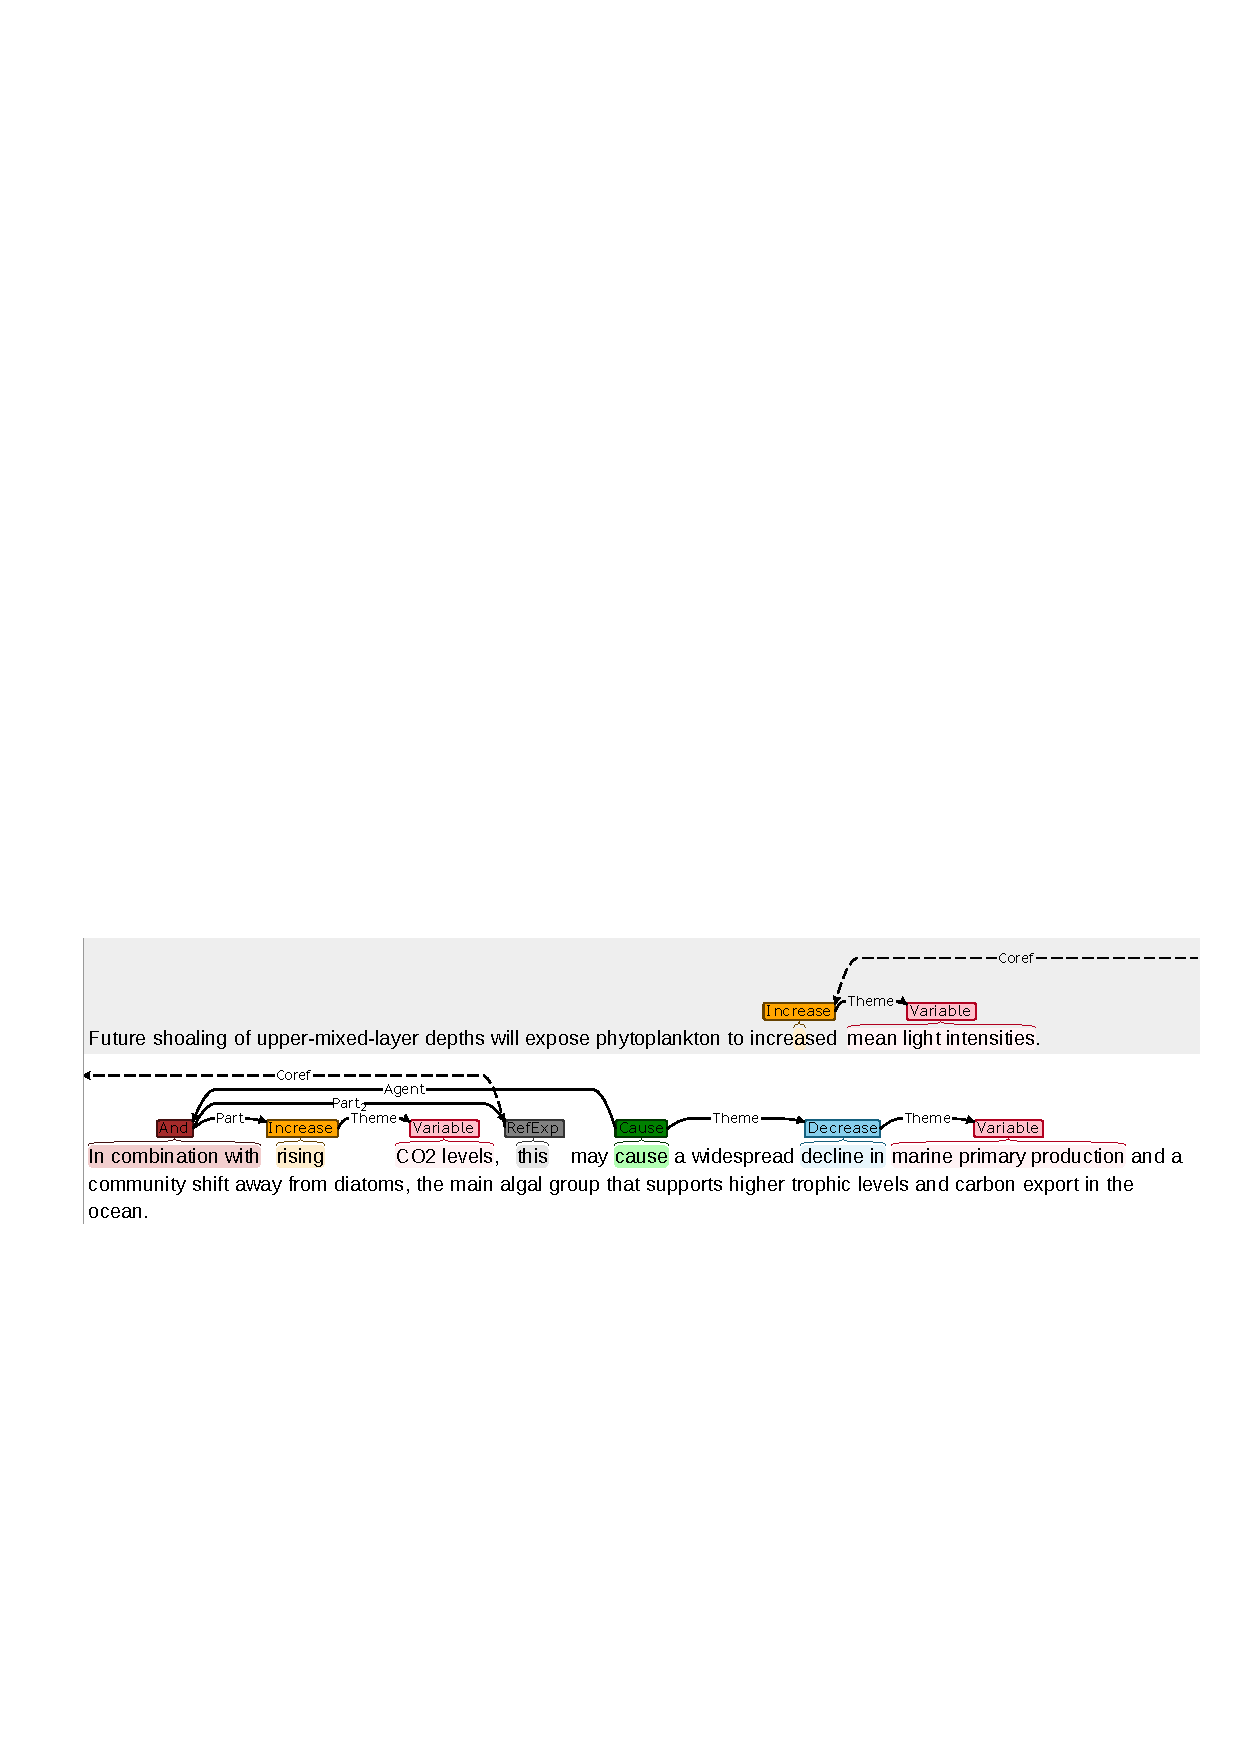
\includegraphics[scale=0.9]{ex1.pdf}}
\framebox[\textwidth]{[ $\uparrow$ mean light intensities $\wedge$ $\uparrow$ CO2 levels ]~~~ $\Longrightarrow$~~~$\downarrow$ marine primary production}
 \caption{Example of a causal rule extracted from a pair of annotated sentences}
\end{center}
\label{fig:ex1}
\end{figure*}


\begin{figure*}
\begin{center}
\framebox[\textwidth]{
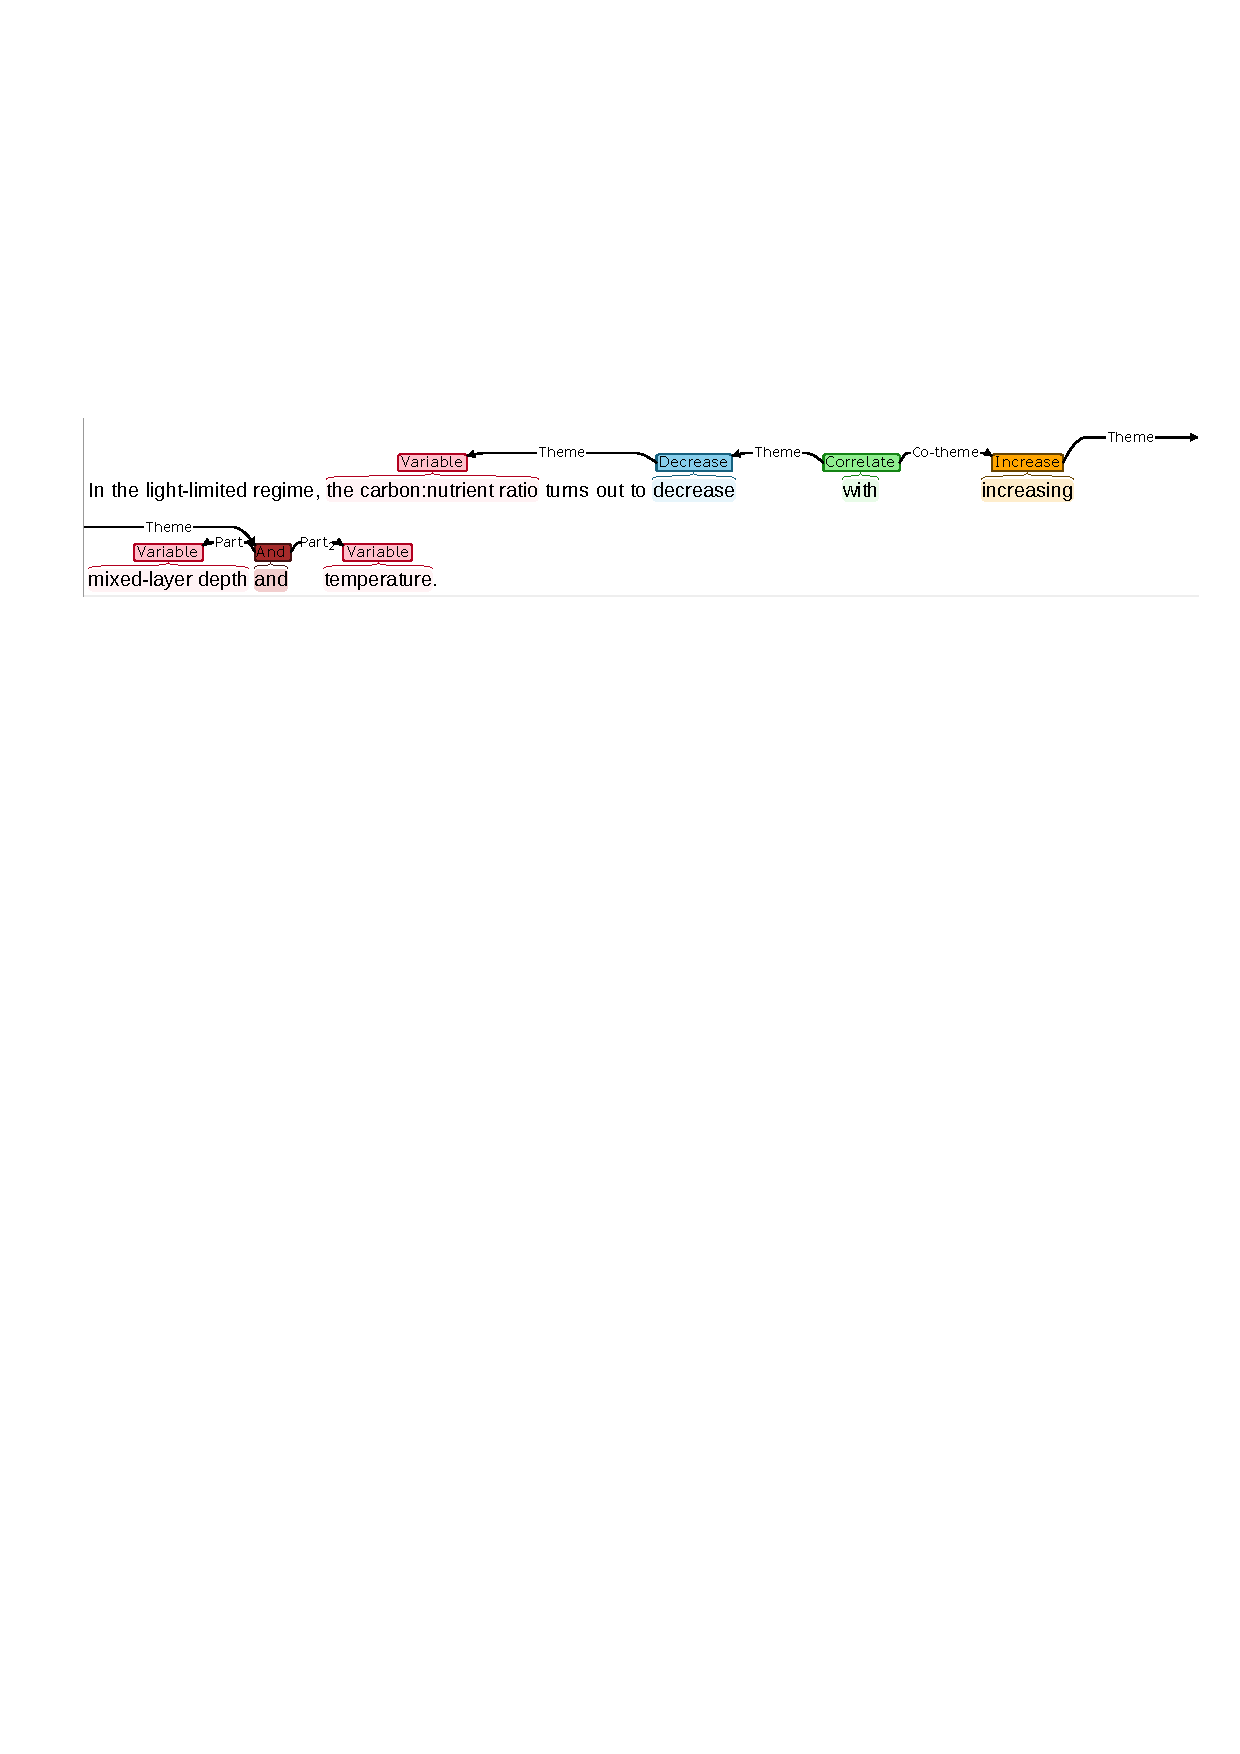
\includegraphics[scale=0.9]{ex2.pdf}}
\framebox[\textwidth]{[ $\uparrow$ mixed-layer depth $\wedge$ $\uparrow$ temperature ]~~~ $\leadsto$~~~$\downarrow$ the carbon:nutrient ratio}
 \caption{Example of a correlation rule extracted from an annotated sentence}
\end{center}
\label{fig:ex2}
\end{figure*}



\begin{figure*}
\begin{center}
\framebox[\textwidth]{
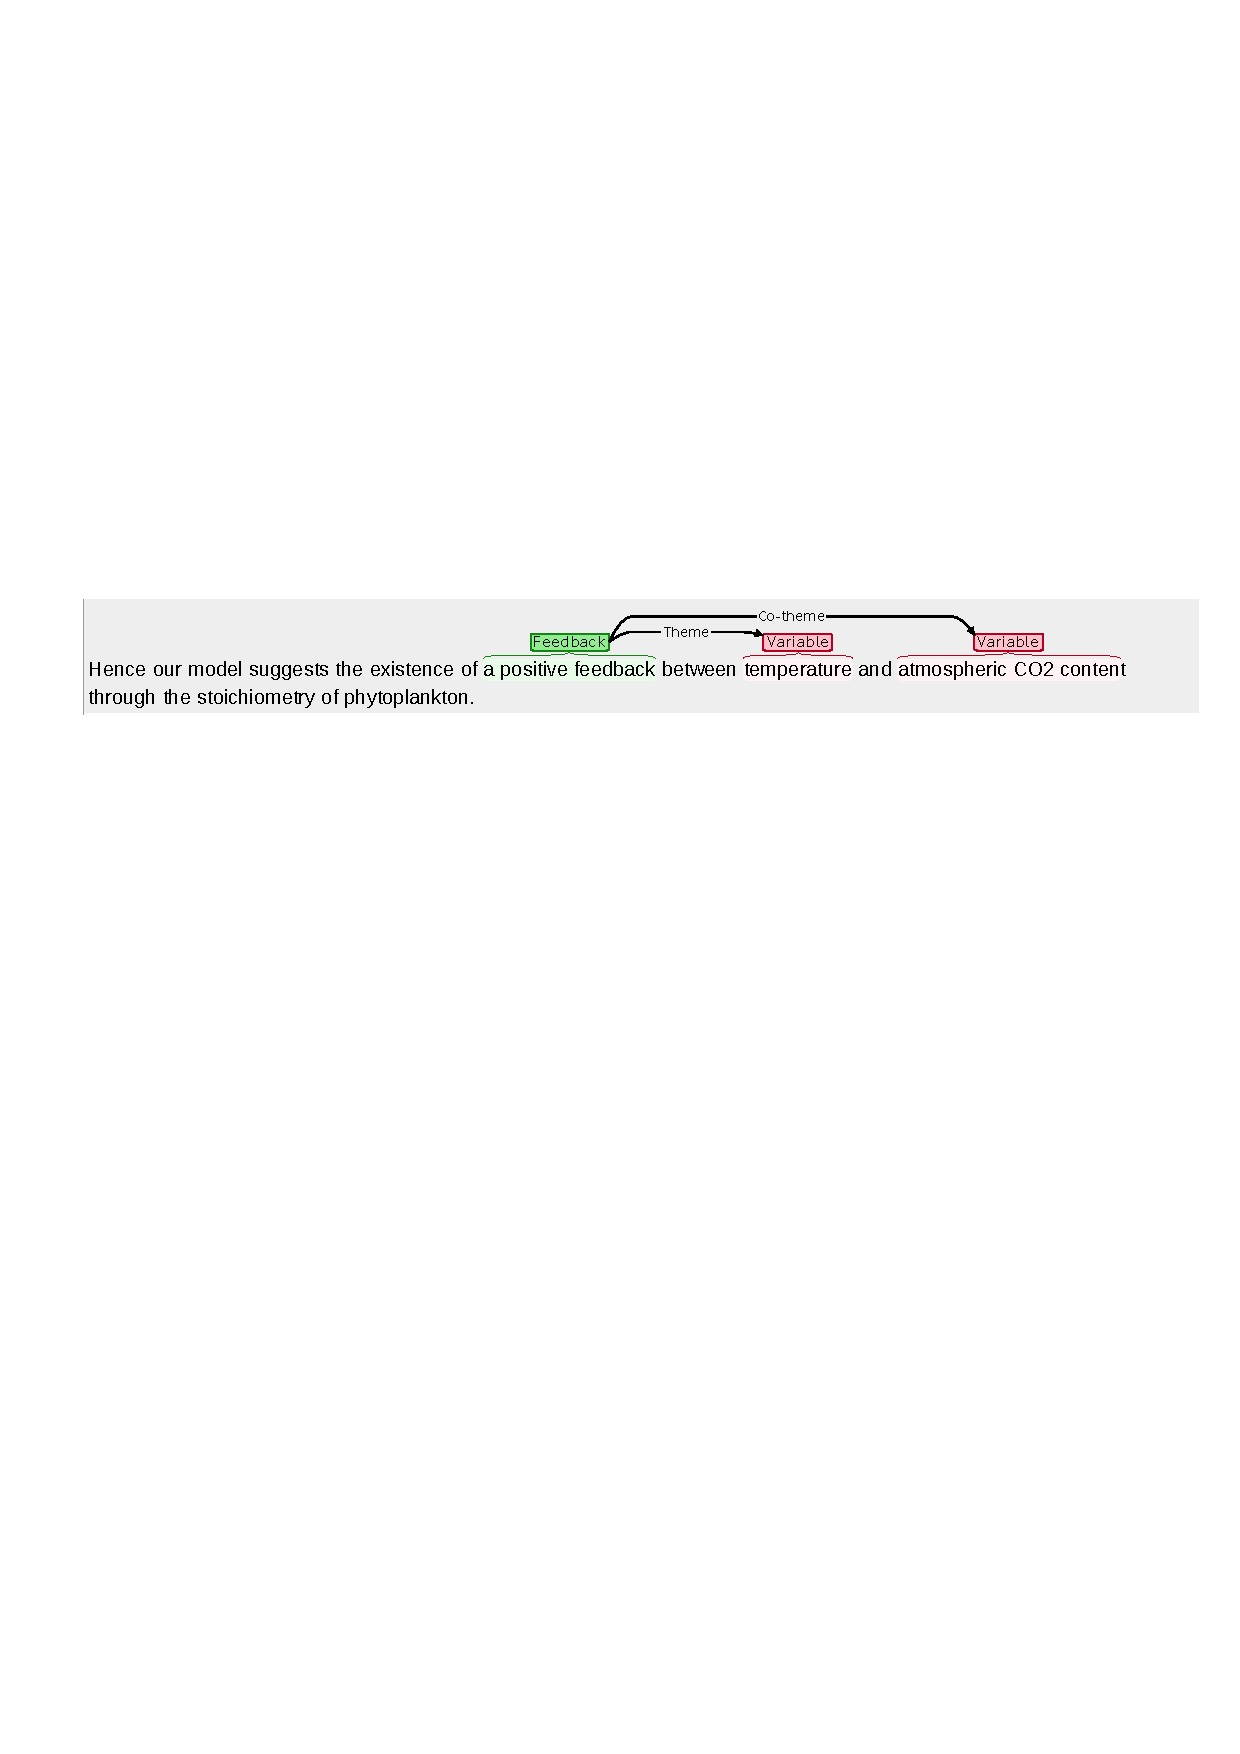
\includegraphics[scale=0.9]{ex3.pdf}}
\framebox[\textwidth]{$\updownarrow$ temperature~~~$\Longleftrightarrow^{+}$~~~$\updownarrow$ marine primary production}
 \caption{Example of a feedback rule extracted from an annotated sentence}
\end{center}
\label{fig:ex3}
\end{figure*}


%=============================================================================
\section{Discussion}
%=============================================================================
\label{sec:discussion}

\todo[inline]{Automatic annotation:
What aproach do we intend to use?
Generic, unsupervised open IE vs dedicated supervised system?
How well do we think this is going to work?
Bootstrapping and active learning to save annotation costs?
}

\todo[inline]{Variables:
Interpretation of variables in context (anaphora resolution and resolving referring expression);
Linking to ontologies
}
In a cross-disciplinary domain such as Environmental/Climate Science, it is likely that different backgrounds lead to differences in vocabulary.
For example, marine chemist use the term \emph{speciation} to describe formation of the different chemical and physical forms of an element, such as organically complexed iron, collidal iron, particulate iron, iron with 2 positive charge (Fe (II)) , iron with 3 positive charge (Fe(III), inorganic iron, etc. 
All of these called \emph{species} of iron and to separate iron forms into these forms is \emph{speciation}. 
In contrast, marine biologist use the term \emph{species} for different forms of life; for example, \emph{diatom} and \emph{dinoflagelattes} are diferent species.

To Swanson link the statements $A \to B_1$ and $B_2 \to C$, it is necessary to for the system to detect that $B_1 = B_2$ given that $B_1$ and $B_2$ are synonymous.
To this end, it will be necessary to link the annotated variables to concepts in a domain ontology\EA{Given that we have an ontology, would this be a part of the annotation process, or simply something we do computational later on?}.

\todo[inline]{Reasoning:
How do want to use the extracted rules for reasoning?
Specification/generalization of rules (relation to natural logic?)
How to combine with bckground knowledge?
}
In their NLP-based LBD system, Bitola, \newcite{Hristovski2008NLPinLBD} define certain Discovery Patterns to guide their search through the concept-relation space. 
A discovery pattern specifies a set of conditions, and a relation that is predicted to hold if the conditions are satisfied. 
One example from their application is the \emph{Maybe\_treats} pattern, which holds between a drug and a disease if they have an opposite effect on a body function or bodily substance. 
In the Bitola system the user navigates through the concept-relation chains manually, but it is conceivable to conduct automatic searches for applications of discovery patterns using sub-graph matching.

While potential treatments are of particular interest to the biomedical domain, feedback loops are particularly interesting in the Climate Science domain. 
The annotation guidelines presented here have been developed with the goal of facilitating discovery of feedback loop candidates, in the way they focus on quantitative changes in variables rather than plain causal relations\footnote{This sentence should maybe be moved to an earlier stage, as it explains our motivation. Also this is neglecting contradictions/other chains.}.

First,  quantitative variables and the various types of events (i.e., change, causal, and correlation) and the correlation and causal relationships among these, as shown in annotation examples, are extracted and learned by the system.  
Then the system will generate scientific hypotheses on the basis of this extracted knowledge. 
A hypothesis is  either 1) a chain of events that connects  different oceanographic entities that don�t appear  together in any of the extracted individual relationships/rules, or  2) a chain that starts and ends with the same entity but does this  through a chain of extracted rules of at least length two.  
The latter type of chains capture discovery hypotheses about the feedback loops which are of key importance for knowledge discovery in  climate science.

Generation of discovery hypotheses is essentially a search on a rather large event and relation space. 
Relations with the left-hand side (LHS) and right-hand side (RHS) representation can be considered as rules and reasoning with the extracted relation will therefore follow a production rule inspired approach. 
The extracted rules comprise the rule base and a working memory(WM) represents the knowledge elements such as events and quantitative variables as well as partially discovered hypotheses, i.e., the parts of  hypothesis chains  so far discovered. 
A rule can �fire�  when its LHS matches the knowledge elements asserted to the working memory.  
When a rule fires, its RHS indicates new knowledge elements to be placed into the WM. In this way, the number of knowledge elements in the WM increases quickly. 
Consequently, there may be several rules, at each step,  of which LHS can match with facts in the WM. Decision of which rule to fire, i.e., "conflict resolution", may increasingly become time demanding. 
To combat the complexity of the search, some heuristic are needed. 
Heuristics need to be formulated according to the peculiarities of the climate domain. 
Just to give an idea, one  concern may be whether the more general or  the more specific rules will be most preferred. 

A rule may be more general than another one when an event it involves subsumes an event in the other rule.  
For example {\it Disease may cause dead"} is more general than {\it Cancer may cause dead}. Similarly,  a rule that have more conjunctions  is more specific than a rule that has no or fewer AND on itsLHS. 
For example, 
{\it Lack of nitrogen causes a decline in phytoplankton growth} rate is more specific than {\it Lack of iron causes a decline in phytoplankton growth rate}. 
For example GRAFFITI \newcite{Fajtlowicz89}  that discovers hypotheses in geometry and conjectures in graph theory prefers more general statements over specific ones. 
ARROWSMITH on the other hand prefers less general conjectures while filtering out broad terms such as �hormone�, because it aims to discover  unknown �positive� side effects of a specific drug. 

The subsumption relation between two event concepts is part of the background knowledge every climate researcher is assumed to have. 
This type of knowledge, therefore, is not explicitly pronounced anywhere in the  climate science literature.
While this is not a problem for human experts,  a computer system needs to represent this background knowledge explicitly and use it, for example, when comparing their generality/specificity. 
Using the example mentioned above, the background knowledge should represent an  IS-A relation between {\it disease} and {\it cancer}, i.e., {\it cancer IS-A disease}. 

Another important use of domain knowledge is during the construction of chains, more specifically, when connecting the RHS of a rule with the LHS of the next rule in the chain. 
Let us assume two rules $A \to B$   and  $C \to D$. 
In some cases B will be the directly equal to C while in other cases there maybe a close but "indirect" relationship between B and C  (e.g., B IS-A F, F PART-OF D,  D IS-A C) which is not explicit in any extracted rule.  
Again, for human experts this may be background knowledge which corresponds to a chain of relations in the domain knowledge of the LBKD system and needs to be derived from the domain knowledge base in order to connect the rules  $A \to B$ and $B \to C$ . 




\todo[inline]{Meta-knowledge and context:
Are there examples where context is essential for proper rule application (conditions?)
}

Another mechanism for narrowing the search, as well as increasing the quality of the discovery chains is to represent the context/constraints specifying when a rule is sanctioned. For example X may cause Y only when the temperature is higher than 10 centigrade degrees. Yet  another mechanism for restricting the search is associating confidence measures to the extracted rules.  Rules that have higher confidence levels are in general given higher priority to be selected. A rule may have higher confidence if it is found in multiple papers compared to a rule that is extracted from only one paper. The type of journal the paper is published also affects the confidence level, i.e, \emph{Nature} or \emph{Science} are presumed to give higher confidence to the papers, and in turn, rules extracted from these papers. 

\todo[inline]{User interface:
What kind of use cases do we imagine?
What functionalities (e.g. clicking through to see source text of rule in publication )
What kind of user interface would support this? 
}
\MVA{For a user interface as a user of potential program  i wish to see
1-around the interaction between the variables of X and Y 
A) to check how other variables will be effected from the interaction between  X and Y 
  B) to check  cascade effects visually
C) to see the most and least significant changes in a visualised way
D) to see conflicting information
E) to see or define contextual restriction
}

The complete system is conceived as a research support system that provides the user with a overview over the relations between the concepts in the domain. 
In the perceived user interface, the user can look up any domain concept.
The user will then be presented with a list of the concepts that are in a relation with the look-up concept. 
By again looking up concepts that are in a relation with the newly selected concept the user can build a chain of related concepts.
The user interface will let the user explore the relation holding between two concepts closely, by providing links to the source sentence(s) from which the relation was extracted. 
Based on the frequency of occurrence of the relation between the two concepts and the source text, the user will the be able to judge the validity of the concept-relation chain.
This should reduce the workload for a researcher by providing easy and comprehensive access to relevant relations in the domain as well as pointers to source texts.

%=============================================================================
\section{Conclusion}
%=============================================================================


\todo[inline]{Conclusions}

%=============================================================================
\section{Acknowledgements}
%=============================================================================

Financial aid from the European Commission (OCEAN-CERTAIN, FP7-ENV-2013-6.1-1; no: 603773) is gratefully acknowledged. 


\bibliographystyle{lrec2006}
\bibliography{biotxtm14}

\end{document}

